\documentclass[a4paper]{article}
\usepackage{graphicx}
\usepackage{amsmath, amsfonts, geometry, float, listings, enumerate, multicol}
\usepackage{multicol, float, color, colortbl}
\usepackage{tikz, titlesec, parskip}

\titlespacing{\section}{0pt}{10pt}{0pt}
\titlespacing{\subsection}{0pt}{10pt}{0pt}
\titlespacing{\subsubsection}{0pt}{10pt}{0pt}

\usetikzlibrary{calc,patterns,through}
\newcommand{\arcangle}{%
	\mathord{<\mspace{-9mu}\mathrel{)}\mspace{2mu}}%
}

\renewcommand{\baselinestretch}{1.2}
 \geometry{
 a4paper,
 total={170mm,257mm},
 left=20mm,
 top=20mm,
 }
\usepackage{fancyhdr}
\pagestyle{fancy}
\fancyhf{}
\rhead{\textbf{مقدمه‌ای بر یادگیری ماشین}}
\lhead{\textbf{تمرین سری هشتم}}
\cfoot{\space \space \space \space \textbf{\thepage}  \space \space \space}
\renewcommand{\headrulewidth}{1pt}
\renewcommand{\footrulewidth}{1pt}
 
\usepackage{xepersian}
%\setlatintextfont{Times New Roman}
\settextfont{XB Niloofar}
\setdigitfont{XB Niloofar}
\DefaultMathsDigits
\usepackage{amsmath}
\usepackage{pgfplots}
\tikzset{declare function={unitstep(\x)=notless(\x,0);}}
\tikzset{declare function={delta(\x)=equal(\x,0);}}

\begin{document}
\begin{minipage}{0.6\textwidth}

\begin{center}
	\begin{bf}
	باسمه تعالی\\
	\vspace{0.25cm}
	دانشگاه صنعتی شریف\\
	\vspace{0.25cm}
	دانشکده مهندسی برق\\
	\vspace{0.5cm}

\large
مقدمه‌ای بر یادگیری ماشین -دکتر سیّد جمال‌الدین گلستانی\\
\vspace{0.3cm}
\normalsize
بهراد منیری - ۹۵۱۰۹۵۶۴\\
\Large
\vspace{0.3cm}
گزارش  تمرین سری هشتم\\
\vspace{0.4cm}

\end{bf}
\end{center}
\end{minipage} \hfill
\begin{minipage}{0.35\textwidth}

\begin{flushleft}
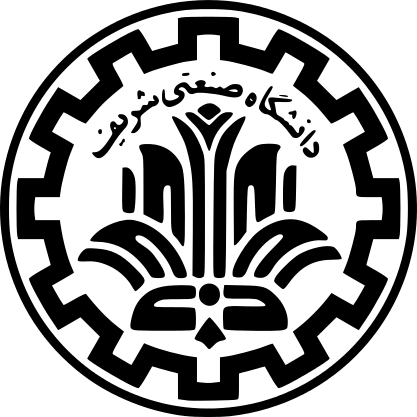
\includegraphics[width=0.6\textwidth]{Shariflogo.png}\\ \large
\end{flushleft}
\end{minipage}

\begin{large}

\part{طبقه‌بندی}
در این بخش به طبقه‌بندی دیتاست معروف 
\lr{Fashion MNIST}
با استفاده از چندین روش مختلف کرده و برای هر روش، پارامتر‌های مربوطه ره به نحوی تنظیم می‌کنیم که بهترین عملکرد ممکن را بر روی داده‌های تست داشته باشیم. نصف داده‌ها به عنوان داده‌ی آموزش و نصف دیگر به عنوان داده‌ی تست استفاده شده است. در کل ۱۰۰۰۰ تصویر در ۱۰ کلاس در اختیار داریم. در انتها نیز روش‌های استفاده‌شده را به یکدیگر مقایسه می‌کنیم. برای هر روش ماتریس کانفیوژن و همچنین درصد کلی عملکرد، آورده شده است.

\section{\lr{Linear SVM}}
پیاده‌سازی 
\lr{SVM}
خطی. در این بخش از تابع
\lr{sklearn.SVC}
استفاده ‌کرده و کرنل را خطی قرار دادیم.

درصد عملکرد کلی این روش
$80.66\%$
است.

\begin{figure}[h!]
	\centering
	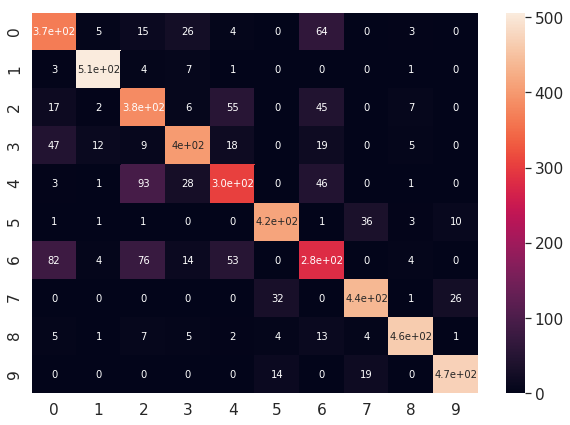
\includegraphics[scale=0.6]{linSVM.png}
	\caption{ماتریس کانفیوژن 
\lr{Linear SVM}	
}
\end{figure}

\section{\lr{Kernel SVM}}
پیاده‌سازی 
\lr{SVM}
با کرنل گاوسی. در این بخش از تابع
\lr{sklearn.SVC}
استفاده ‌کرده و کرنل را \lr{RBF} قرار دادیم. همچنین 
$$C = 10^6 ,\;\;\;\;\gamma = 2\times {10}^{-7}$$
با آزمون و خطا به عنوان پارامتر‌های ما انتخاب شدند.

درصد عملکرد کلی این روش
$86.88\%$
است.

\begin{figure}[h!]
	\centering
	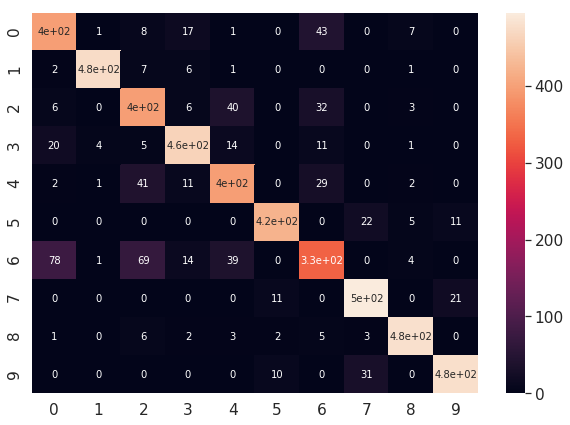
\includegraphics[scale=0.6]{RBFSVM.png}
	\caption{ماتریس کانفیوژن 
		\lr{Kernel SVM}	
	}
\end{figure}
\newpage
\section{\lr{kNN}}
در این بخش با 
\lr{k-Nearest Neighbor }
به طبقه‌بندی می‌پردازیم. 
$$k = 6$$
با آزمون و خطا به عنوان پارامتر‌ انتخاب شد.

درصد عملکرد کلی این روش
$79.94\%$
است.

\begin{figure}[h!]
	\centering
	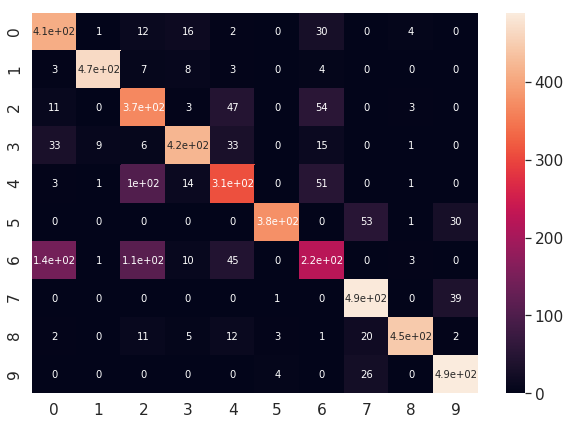
\includegraphics[scale=0.6]{kNN.png}
	\caption{ماتریس کانفیوژن 
		\lr{kNN}	
	}
\end{figure}

\newpage
\section{\lr{Decision Tree}}
در این بخش از 
\lr{Decision Tree}
برای طبقه‌بندی استفاده شده است. درصد عملکرد کلی این روش
$73.06\%$
است.

\begin{figure}[h!]
	\centering
	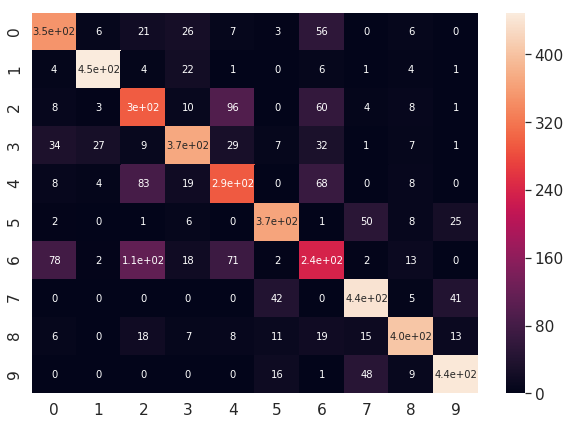
\includegraphics[scale=0.6]{DT.png}
	\caption{ماتریس کانفیوژن 
		\lr{Decision Tree}	
	}
\end{figure}

\newpage
\section{\lr{MLP with Adam Optimizer}}
در این بخش یک شبکه‌ی 
\lr{Multi-Layer Preceptron}
با دو لایه‌ی مخفی که هر کدام ۱۰۰ نورون دارند آموزش داده‌ می‌شود. تابع 
\lr{Activation}
این نورون‌ها 
\lr{ReLU}
 انتخاب شده است ولی به‌جای 
 \lr{SGD}
 از الگوریتم 
 \lr{Adam}
 برای بهینه‌سازی استفاده شده است. تابع تلف به صورت پیش‌فرض
 \lr{Cross Entropy}
 است.

  درصد عملکرد این روش 
 $80.14 \%$
 است.
\begin{figure}[h!]
	\centering
	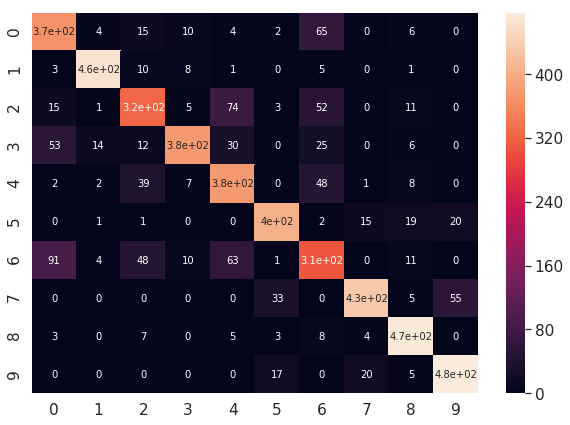
\includegraphics[scale=0.6]{adam.png}
	\caption{ماتریس کانفیوژن 
		\lr{MLP}	
		با 
	 \lr{Adam}
	}
\end{figure}
شکل زیر، تغییرات تابع تلف را در تکرارهای الگوریتم بهینه‌سازی مشاهده می‌کنید.
\begin{figure}[h!]
	\centering
	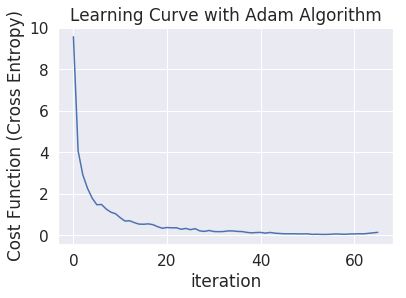
\includegraphics[scale=0.6]{adam2.png}
	\caption{
		\lr{Learning Curve of MLP with Adam Algorithm}
	}
\end{figure}

\newpage
\section{\lr{MLP with SGD Optimizer}}
در این بخش یک شبکه‌ی 
\lr{Multi-Layer Preceptron}
با دو لایه‌ی مخفی که هر کدام ۱۰۰ نورون دارند آموزش داده‌ می‌شود. تابع 
\lr{Activation}
این نورون‌ها 
\lr{tanh}
انتخاب شده است. برای بهینه‌سازی از الگوریتم 
\lr{SGD}
استفاده شده است. تابع تلف به صورت پیش‌فرض
\lr{Cross Entropy}
است.

  درصد عملکرد این روش 
$76.96 \%$
است.
\begin{figure}[h!]
	\centering
	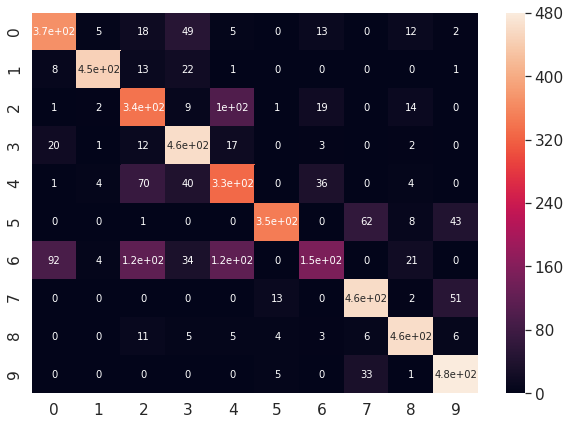
\includegraphics[scale=0.6]{sgd.png}
	\caption{ماتریس کانفیوژن 
		\lr{MLP}	
		با 
		\lr{SGD}
	}
\end{figure}
شکل زیر، تغییرات تابع تلف را در تکرارهای الگوریتم بهینه‌سازی مشاهده می‌کنید.
\begin{figure}[h!]
	\centering
	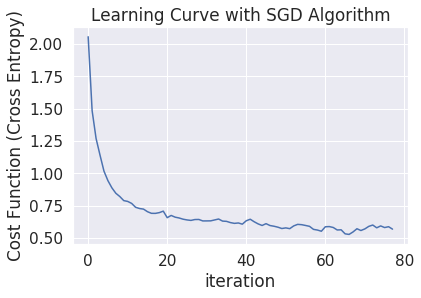
\includegraphics[scale=0.6]{sgd2.png}
	\caption{
		\lr{Learning Curve of MLP with SGD Algorithm}
	}
\end{figure}
\newpage


\section{مقایسه روش‌های طبقه‌بندی}
جدول زیر نتایج طبقه‌بندی روش‌های مختلف را در کنار هم‌دیگر آورده است.
\begin{center}
\begin{table}[h!]
	\centering
	\begin{latin}
	\begin{tabular}{|c|c|c|}
		
				\hline
				\rowcolor[HTML]{C0C0C0} 
		Method        & Params                                                                                             & Accuracy \\
				\hline
		Linear SVM    & -                                                                                                  & 80.66\%  \\
		
		\hline
		Kernel SVM    &$ C= 10\;\;\gamma = 2\times 10^{-7}$ & 86.88\%  \\				\hline
		kNN           & k = 6                                                                                              & 79.94\%  \\
				\hline
		Decision Tree & -                                                                                                  & 73.06\%  \\
				\hline
		MLP (Adam)    & ReLU                                                                                               & 80.14\%  \\
				\hline
		MLP (SGD)     & tanh                                                                                               & 76.96\% \\
				\hline
	\end{tabular}
\end{latin}
\caption{مقایسه‌ی عملکرد روش‌های طبقه‌بندی }
\end{table}
\end{center}

بهترین عملکرد کلی را روش 
\lr{Kernel SVM}
داشت. این روش در مقایسه با روش ‌های مانند 
\lr{kNN}
از سرعت یادگیری بالاتری نیز برخوردار بود. اشتباه بین لیبل صفر و شش (پیراهن و تی‌شرت) بسیار شایع بود در حالی که این اشتباه تا حد زیادی در روش 
\lr{Kernel SVM}
حل شده بود.  این روش به شدت به پارامتر
$\gamma$
وابسته است و مقدار آن با دقت فراوانی تنظیم شده است.


در یادگیری شبکه‌‌عصبی، مشاهده شده که استفاده از الگوریتم 
\lr{Adam}
به جای 
\lr{SGD}
باعث می‌شود به نقطه‌ی بهینه‌تری برسم فلذا نتایج این روش نیز در گزارش آمده است.
\part{خوشه‌بندی}
\section{پیاده‌سازی 
\lr{K-Means}
}

در ابتدا به پیاده‌سازی الگوریتم 
\lr{K-Means}
می‌پردازیم. این الگوریتم به این نحو عمل می‌کند که در ابتدا نقاطی به صورت تصادفی به عنوان مرکز خوشه‌ها انتخاب می‌وند و سپس به صورت تکراری، یک نقطه تصادفی انتخاب می‌شود و فاصله‌ی آن با مراکز دسته‌ها سنجیده می‌شود و در صورتی که دسته‌ای وجود داشته باشد که مرکز آن به این نقطه از مرکز دسته‌ای که هم‌اکنون نقطه در آن قرار دارد نزدیک‌تر باشد، نقطه به دسته‌ی مذکور اضافه می‌شود و سپس مرکز دسته‌ها بروزرسانی می‌شوند. پیاده‌سازی این الگوریتم بر پایه‌ی 
\lr{numpy}
در پایتون انجام شد.


\section{خوشه‌بندی 
\lr{iris}
}
در این بخش به خوشه‌بندی دیتاست معروف 
\lr{iris}
می‌پردازیم. در این مرحله، از هر چهار ویژگی برای خوشه‌بندی استفاده می‌کنیم. برای خوشه‌بندی از 
\lr{K-Means}
استفاده می‌کنیم که در آن 
$k=3$
قرار دادیم. 
\begin{figure}
	\centering
	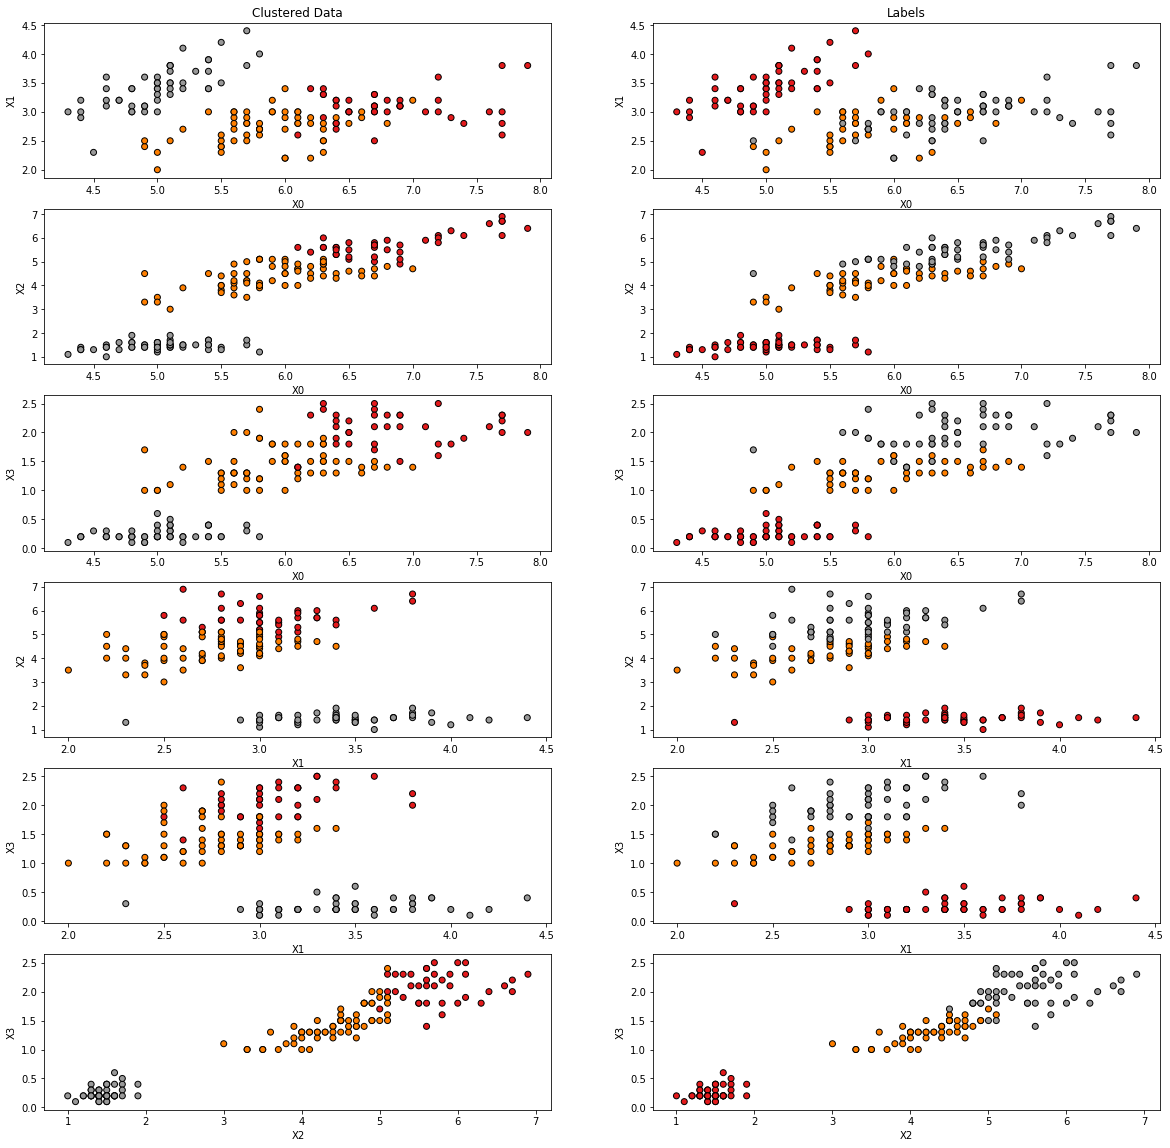
\includegraphics[scale=0.4]{cluster4.png}
	\caption{برسی خوشه‌بندی - نمودار سمت راست بر حسب لیبل‌های واقعی و نمودار سمت چپ بر اساس خوشه‌بندی است}
	\label{cluster4}
\end{figure}

نکته‌ی بسیار جالب این است که این خوشه‌بندی بسیار شبیه به لیبل‌های واقعی نوع گل است در حالی که این نحوه‌ی یادگیری 
\lr{unsupervised}
است. شکل 
\eqref{cluster4}
خروجی این خوشه‌بندی (سمت چپ) و همچنین لیبل‌های واقعی (سمت راست) را نشان می‌دهد. تطابق زیادی بین هر دو نمودار دیده‌ می‌شود. در حال که لزومی نداشت این اتفاق بیافتد.


\section{حذف یک ویژگی}
در این بخش قصد داریم یک ویژگی را حذف کنیم و بررسی کنیم که آیا حذف این ویژگی تاثیر معناداری بر خوشه‌بندی ما دارد یا خیر. هر بار یکی از ویژگی‌ها را حذف کرده و نتایج خوشه‌بندی را در این گزارش درج می‌کنیم.


\subsection{حذف 
	\lr{Sepal Width}
}
در این بخش ویژگی 
	\lr{Sepal Width}
	را حذف و سپس خوشه‌بندی می‌کنیم.
	در شکل
	\eqref{f1}
	نمودار های سمت چپ مربوط به نتایج خوشه‌بندی و نمودار‌های سمت  راست مربوط به لیبل‌های واقعی گل‌هاست. صحت خوشه‌بندی تغییر محسوسی نیافته است.

\begin{figure}[h!]
	\centering
	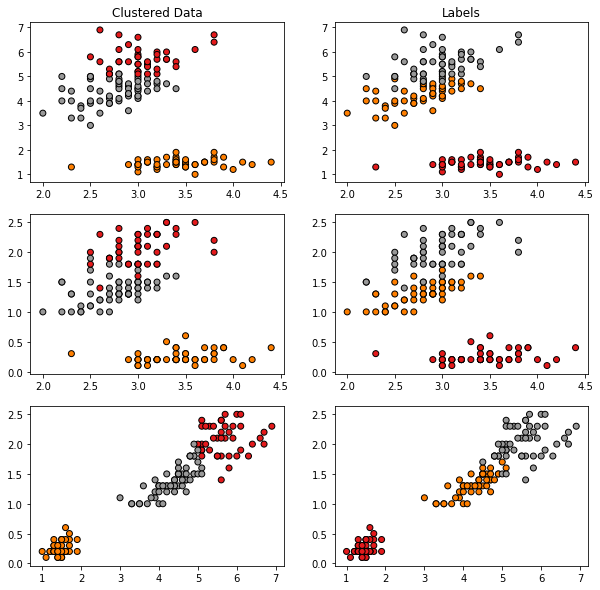
\includegraphics[scale=0.6]{f1.png}
	\caption{برسی خوشه‌بندی - نمودار سمت راست بر حسب لیبل‌های واقعی و نمودار سمت چپ بر اساس خوشه‌بندی 
		است. در این‌جا ویژگی  
			\lr{Sepal Width}
			حذف شده است.
	}
	\label{f1}
\end{figure}

\newpage
\subsection{حذف 
	\lr{Sepal Length}
}
در این بخش ویژگی 
\lr{Sepal Length}
را حذف و سپس خوشه‌بندی می‌کنیم.
در شکل
\eqref{f2}
نمودار های سمت چپ مربوط به نتایج خوشه‌بندی و نمودار‌های سمت  راست مربوط به لیبل‌های واقعی گل‌هاست. صحت خوشه‌بندی تغییر محسوسی نیافته است.
\begin{figure}[h!]
	\centering
	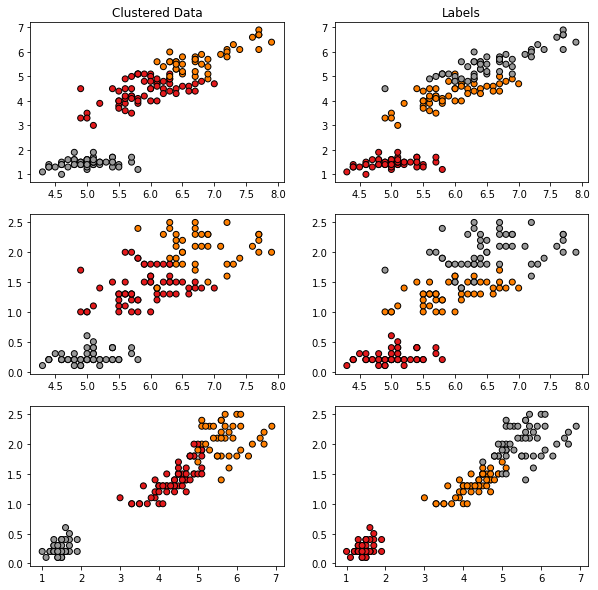
\includegraphics[scale=0.6]{f2.png}
	\caption{برسی خوشه‌بندی - نمودار سمت راست بر حسب لیبل‌های واقعی و نمودار سمت چپ بر اساس خوشه‌بندی 
		است. در این‌جا ویژگی  
		\lr{Sepal Length}
		حذف شده است.
	}
	\label{f2}
\end{figure}
\newpage
\subsection{حذف 
	\lr{Petal Length}
}
در این بخش ویژگی 
\lr{Petal Length}
را حذف و سپس خوشه‌بندی می‌کنیم.
در شکل
\eqref{f3}
نمودار های سمت چپ مربوط به نتایج خوشه‌بندی و نمودار‌های سمت  راست مربوط به لیبل‌های واقعی گل‌هاست. صحت خوشه‌بندی تغییر محسوسی نیافته است.
\begin{figure}[h!]
	\centering
	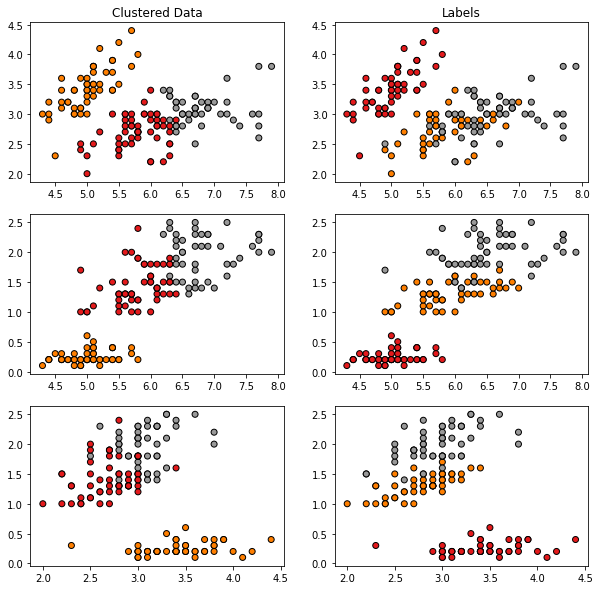
\includegraphics[scale=0.6]{f3.png}
	\caption{برسی خوشه‌بندی - نمودار سمت راست بر حسب لیبل‌های واقعی و نمودار سمت چپ بر اساس خوشه‌بندی 
		است. در این‌جا ویژگی  
		\lr{Petal Length}
		حذف شده است.
	}
	\label{f3}
\end{figure}

\newpage
\subsection{حذف 
	\lr{Petal Width}
}
در این بخش ویژگی 
\lr{Petal Width}
را حذف و سپس خوشه‌بندی می‌کنیم.
در شکل
\eqref{f3}
نمودار های سمت چپ مربوط به نتایج خوشه‌بندی و نمودار‌های سمت  راست مربوط به لیبل‌های واقعی گل‌هاست. صحت خوشه‌بندی تغییر محسوسی نیافته است.
\begin{figure}[h!]
	\centering
	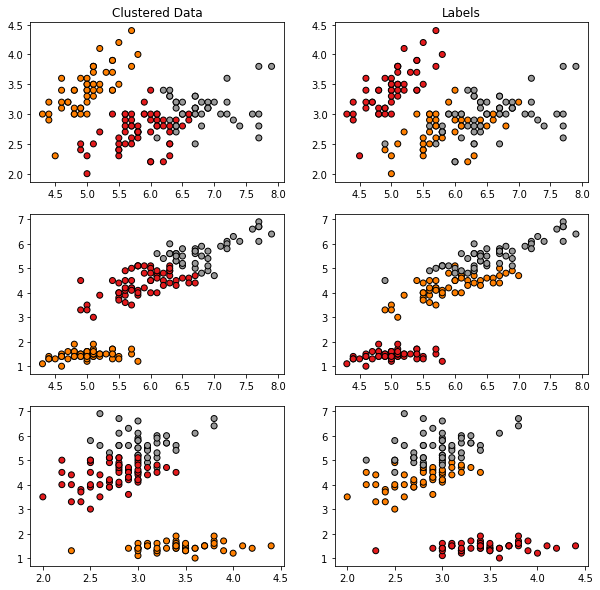
\includegraphics[scale=0.6]{f4.png}
	\caption{برسی خوشه‌بندی - نمودار سمت راست بر حسب لیبل‌های واقعی و نمودار سمت چپ بر اساس خوشه‌بندی 
		است. در این‌جا ویژگی  
		\lr{Petal Width}
		حذف شده است.
	}
	\label{f4}
\end{figure}
\newpage
\section{بررسی تغییرات مراکز خوشه‌ها}
در این بخش، با تغییر کد الگوریتم 
\lr{K-Means}
در هر مرحله، مراکز خوشه‌ها را ذخیره کرده و در انتها مسیر حرکت آن‌ها را در طی تکرار‌ها رسم می‌کنیم. در این‌جا ما تنها از دو ویژگی 
\lr{Petal Width}
و 
\lr{Petal Length}
استفاده می‌کنیم. در شکل 
\eqref{fin}
و 
\eqref{fin2}
خروجی خوشه‌بندی و همچنین مسیر حرکت مراکز خوشه‌ها را مشاهده می‌کنید.
\begin{figure}[h!]
	\centering
	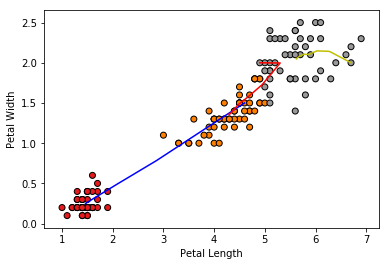
\includegraphics[scale=0.6]{fin.png}
	\caption{بررسی تغییرات مراکز خوشه‌ها}
	\label{fin}
\end{figure}
\begin{figure}[h!]
	\centering
	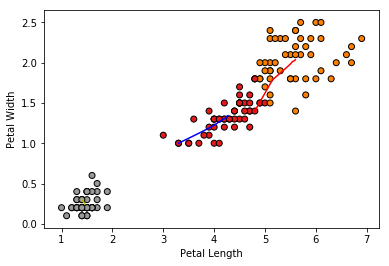
\includegraphics[scale=0.6]{fin2.png}
	\caption{بررسی تغییرات مراکز خوشه‌ها}
	\label{fin2}
\end{figure}


\end{large}
\end{document}